%%=============================================================================
%% Onderzoek
%%=============================================================================

\chapter{Vergelijkend Onderzoek}
\label{ch:vergelijkendonderzoek}
In dit deel van het onderzoek zal er van de twee eerder opgebouwde datamodellen een vergelijking gemaakt worden. Hierbij wordt voornamelijk gefocust op deze 5 pijlers:

\begin{itemize}
	\item \textbf{Performantie:} is er een significant verschil in het uitvoeren van leesopdrachten?
	\item \textbf{Complexiteit:} zijn beide modellen makkelijk interpreteerbaar door IT \& business?
	\item \textbf{Flexibiliteit:} hoe flexibel zijn beide modellen wanneer een business requirement gewijzigd wordt?
	\item \textbf{Schaalbaarheid:} hoe gaan beide modellen overweg met het inladen van enorme hoeveelheid data?
	\item \textbf{Audit:} is er metadata beschikbaar over de werkelijke data? Kunnen problemen makkelijk opgespoord worden?
\end{itemize} 

Op basis van deze resultaten zal er kunnen opgemaakt worden of de keuze voor Data Vault wel de juiste keuze was voor dit project.

\section{Performantie}
In deze sectie wordt het vergelijkend onderzoek gestart door de performantie bij leesopdrachten te vergelijken tussen Data Vault en het dimensioneel model. Voor het verkrijgen van de resultaten wordt een procedure geschreven in SQL-code die de executietijd zal berekenen. Elke query zal 1000 keer uitgevoerd worden. Op basis van de verkregen resultaten kan er een correcte analyse opgemaakt worden. Deze queries worden uitgevoerd op een \textbf{SAP HANA databank}, door het gebruik te maken van deze technologie zal dit een invloed hebben op de snelheid van executie. Zowel voor Data Vault als voor het dimensioneel werden de leesopdrachten uitgevoerd met 2 verschillende hoeveelheden van data. De 1000 leesoperaties werden uitgevoerd op 1200 en 100.000 records waarbij alle tabellen van ieder model opgevraagd worden. Al deze opgehaalde data zou dan kunnen gebruikt worden voor het opmaken van dashboards.

\subsection{Procedure} 
\lstset{breaklines=true,keywordstyle=\bfseries\color{blue!40!black}}
\begin{lstlisting}[frame=single] 
CREATE PROCEDURE "TESTJORIK_BV"."RESULTS" LANGUAGE SQLSCRIPT AS BEGIN

--Declareren van variabele (teller)
DECLARE EXEC_ID int;

--Initialiseren van variabele
EXEC_ID = 1;

--Starten van loop (1000x queries uitvoeren)
WHILE :EXEC_ID < 1001 DO

--ID toevoegen in databank
INSERT INTO "TESTJORIK_BV"."UITVOERINGSTIJDEN" ("EXEC_ID") VALUES (:EXEC_ID);

--Tijdstip van start toevoegen in de databank voor het Data Vault model
UPDATE "TESTJORIK_BV"."UITVOERINGSTIJDEN" SET "START_TIME_DV" = CURRENT_TIMESTAMP
WHERE "EXEC_ID" = :EXEC_ID;

--Uitvoeren query leesopdracht op DataVault model
SELECT hubarticle."ARTICLE_ID", hubwarehouse."WAREHOUSE_ID", hubstatus."STATUS_ID", hubstaff."STAFF_ID", hubpallet."PALLET_ID", hubdelivery."DELIVERY_ID",
hubgroup."LABO_GROUP_ID", hubentity."LABO_ENTITY_ID", satgroup."LABO_GROUP_NAME", satentity."LABO_ENTITY_NAME", satstaff."STAFF_NAME", satwarehouse."WAREHOUSE_CITY",
satarticle."ARTICLE_NAME", satstatus."STATUS_NAME", hubdock."DOCK_TIME", hubstock."STOCK_TIME", satdts."STOCKED_TOTAL", satdts."STOCKED_WITHIN_12HOURS_QUANTITY",
satdts."STOCKED_WITHIN_16HOURS_QUANTITY", satdts."STOCKED_WITHIN_24HOURS_QUANTITY", satdts."SECONDS_TO_LATE", satdts."SECONDS_BETWEEN_STOCK_AND_DOCK", satorderline."ARTICLE_QUANTITY"
FROM "BP_DHLPL_RAWDATAVAULT"."LINK_DOCK_TO_STOCK" as linkdts
INNER JOIN "BP_DHLPL_RAWDATAVAULT"."HUB_DOCK" as hubdock
ON linkdts."DOCK_HASH_KEY" = hubdock."DOCK_HASH_KEY"
INNER JOIN "BP_DHLPL_RAWDATAVAULT"."HUB_STOCK" as hubstock
ON linkdts."STOCK_HASH_KEY" = hubstock."STOCK_HASH_KEY"
INNER JOIN "BP_DHLPL_RAWDATAVAULT"."HUB_PALLET" as hubpallet
ON linkdts."PALLET_HASH_KEY" = hubpallet."PALLET_HASH_KEY"
INNER JOIN "BP_DHLPL_RAWDATAVAULT"."HUB_STATUS" as hubstatus
ON linkdts."STATUS_HASH_KEY" = hubstatus."STATUS_HASH_KEY"
INNER JOIN "BP_DHLPL_RAWDATAVAULT"."HUB_STAFF" as hubstaff
ON linkdts."STAFF_HASH_KEY" = hubstaff."STAFF_HASH_KEY"
INNER JOIN "BP_DHLPL_RAWDATAVAULT"."LINK_ORDERLINE" as linkorderline
ON hubpallet."PALLET_HASH_KEY" = linkorderline."PALLET_HASH_KEY"
INNER JOIN "BP_DHLPL_RAWDATAVAULT"."HUB_ARTICLE" as hubarticle
ON linkorderline."ARTICLE_HASH_KEY" = hubarticle."ARTICLE_HASH_KEY"
INNER JOIN "BP_DHLPL_RAWDATAVAULT"."LINK_WAREHOUSE_STAFF" as linkwarehousestaff
ON hubstaff."STAFF_HASH_KEY" = linkwarehousestaff."STAFF_HASH_KEY"
INNER JOIN "BP_DHLPL_RAWDATAVAULT"."HUB_WAREHOUSE" as hubwarehouse
ON linkwarehousestaff."WAREHOUSE_HASH_KEY" = hubwarehouse."WAREHOUSE_HASH_KEY"
INNER JOIN "BP_DHLPL_RAWDATAVAULT"."LINK_TRANSPORT" as linktransport
ON hubdock."DOCK_HASH_KEY" = linktransport."DOCK_HASH_KEY"
INNER JOIN "BP_DHLPL_RAWDATAVAULT"."HUB_LABO_ENTITY" as hubentity
ON linktransport."LABO_ENTITY_HASH_KEY" = hubentity."LABO_ENTITY_HASH_KEY"
INNER JOIN "BP_DHLPL_RAWDATAVAULT"."HUB_DELIVERY" as hubdelivery
ON linktransport."DELIVERY_HASH_KEY" = hubdelivery."DELIVERY_HASH_KEY"
INNER JOIN "BP_DHLPL_RAWDATAVAULT"."LINK_LABO_ENTITY_GROUP" as linklabo
ON hubentity."LABO_ENTITY_HASH_KEY" = linklabo."LABO_ENTITY_HASH_KEY"
INNER JOIN "BP_DHLPL_RAWDATAVAULT"."HUB_LABO_GROUP" as hubgroup
ON linklabo."LABO_GROUP_HASH_KEY" = hubgroup."LABO_GROUP_HASH_KEY"
INNER JOIN "BP_DHLPL_RAWDATAVAULT"."SAT_LABO_GROUP" as satgroup
ON satgroup."LABO_GROUP_HASH_KEY" = hubgroup."LABO_GROUP_HASH_KEY"
INNER JOIN "BP_DHLPL_RAWDATAVAULT"."SAT_LABO_ENTITY" as satentity
ON satentity."LABO_ENTITY_HASH_KEY" = hubentity."LABO_ENTITY_HASH_KEY"
INNER JOIN "BP_DHLPL_RAWDATAVAULT"."SAT_STATUS" as satstatus
ON hubstatus."STATUS_HASH_KEY" = satstatus."STATUS_HASH_KEY"
INNER JOIN "BP_DHLPL_RAWDATAVAULT"."SAT_STAFF" as satstaff
ON hubstaff."STAFF_HASH_KEY" = satstaff."STAFF_HASH_KEY"
INNER JOIN "BP_DHLPL_RAWDATAVAULT"."SAT_WAREHOUSE" as satwarehouse
ON hubwarehouse."WAREHOUSE_HASH_KEY" = satwarehouse."WAREHOUSE_HASH_KEY"
INNER JOIN "BP_DHLPL_RAWDATAVAULT"."SAT_ARTICLE" as satarticle
ON hubarticle."ARTICLE_HASH_KEY" = satarticle."ARTICLE_HASH_KEY"
INNER JOIN "BP_DHLPL_RAWDATAVAULT"."SAT_ORDERLINE" as satorderline
ON linkorderline."ORDERLINE_HASH_KEY" = satorderline."ORDERLINE_HASH_KEY"
INNER JOIN "BP_DHLPL_RAWDATAVAULT"."SAT_DOCK_TO_STOCK" as satdts
ON linkdts."DOCK_TO_STOCK_HASH_KEY" = satdts."DOCK_TO_STOCK_HASH_KEY";

--Tijdstip van einde toevoegen in de databank voor het Data Vault model
UPDATE "TESTJORIK_BV"."UITVOERINGSTIJDEN" SET "END_TIME_DV" = CURRENT_TIMESTAMP
WHERE "TESTJORIK_BV"."UITVOERINGSTIJDEN"."EXEC_ID" = :EXEC_ID;

--Tijdstip van start toevoegen in de databank voor het dimensioneel model
UPDATE "TESTJORIK_BV"."UITVOERINGSTIJDEN" SET "START_TIME_DM" = CURRENT_TIMESTAMP
WHERE "TESTJORIK_BV"."UITVOERINGSTIJDEN"."EXEC_ID" = :EXEC_ID;

--Uitvoeren query leesop^dracht op het dimensioneel model 
SELECT fct.*, dimarticle."ARTICLE_NAME", dimentity."LABO_ENTITY_NAME", dimgroup."LABO_GROUP_NAME", dimdelivery."STOCK_TIME", dimdelivery."DOCK_TIME", dimstaff."STAFF_NAME", dimstatus."STATUS_NAME", dimwarehouse."WAREHOUSE_CITY"
FROM "BP_DHLPL_DATAWAREHOUSELAAG"."FACT_DOCKTOSTOCK" as fct
INNER JOIN "BP_DHLPL_DATAWAREHOUSELAAG"."DIM_ARTICLE" as dimarticle
ON fct."ARTICLE_ID" = dimarticle."ARTICLE_ID"
INNER JOIN "BP_DHLPL_DATAWAREHOUSELAAG"."DIM_LABO_ENTITY" as dimentity
ON fct."LABO_ENTITY_ID" = dimentity."LABO_ENTITY_ID"
INNER JOIN "BP_DHLPL_DATAWAREHOUSELAAG"."DIM_LABO_GROUP" as dimgroup
ON fct."LABO_GROUP_ID" = dimgroup."LABO_GROUP_ID"
INNER JOIN "BP_DHLPL_DATAWAREHOUSELAAG"."DIM_DELIVERY" as dimdelivery
ON fct."PALLET_ID" = dimdelivery."PALLET_ID"
INNER JOIN "BP_DHLPL_DATAWAREHOUSELAAG"."DIM_STAFF" as dimstaff
ON fct."STAFF_ID" = dimstaff."STAFF_ID"
INNER JOIN "BP_DHLPL_DATAWAREHOUSELAAG"."DIM_STATUS" as dimstatus
ON fct."STATUS_ID" = dimstatus."STATUS_ID"
INNER JOIN "BP_DHLPL_DATAWAREHOUSELAAG"."DIM_WAREHOUSE" as dimwarehouse
ON fct."WAREHOUSE_ID" = dimwarehouse."WAREHOUSE_ID";

--Tijdstip van einde toevoegen in de databank voor het dimensioneel model
UPDATE "TESTJORIK_BV"."UITVOERINGSTIJDEN" SET "END_TIME_DM" = CURRENT_TIMESTAMP
WHERE "TESTJORIK_BV"."UITVOERINGSTIJDEN"."EXEC_ID" = :EXEC_ID;

--Berekenen van executietijd voor het Data Vault model
UPDATE "TESTJORIK_BV"."UITVOERINGSTIJDEN" SET "DIFF_TIME_DV" = (NANO100_BETWEEN(START_TIME_DV,END_TIME_DV) / 10000)
WHERE "TESTJORIK_BV"."UITVOERINGSTIJDEN"."EXEC_ID" = :EXEC_ID;

--Berekenen van executietijd voor het dimensioneel model
UPDATE "TESTJORIK_BV"."UITVOERINGSTIJDEN" SET "DIFF_TIME_DM" = (NANO100_BETWEEN(START_TIME_DM,END_TIME_DM) / 10000)
WHERE "TESTJORIK_BV"."UITVOERINGSTIJDEN"."EXEC_ID" = :EXEC_ID;

--Waarde teller verhogen met 1
EXEC_ID = :EXEC_ID + 1;
END WHILE;
END;
\end{lstlisting}

\subsection{Resultaten}
Na het doorlopen van de vorige procedure, kan er gestart worden met het vergelijken van de gegenereerde data over de performantie bij leesopdrachten. In tabel \ref{tab:mem} wordt een overzicht getoont van het werkgeheugen die SAP HANA toewees voor het uitvoeren van beide queries (door de query 1 keer uit te voeren). 

\begin{center}
	\renewcommand{\arraystretch}{2}%
	\begin{longtable}{  l  p{4,5cm}  p{4,5cm} }
	    \ & \textbf{Data Vault} & \textbf{Dimensioneel model} \\ \hline
		\textbf{1200 records} & 5,2 MByte(s) & 2,5 MByte(s) \\ \hline
		\textbf{100.000 records} & 139,8 MByte(s) & 4,6 MByte(s) \\
		\caption{Overzicht van het toegewezen werkgeheugen van beide select-statements (verkregen via het Execution plan in SAP HANA).}
		\label{tab:mem}
	\end{longtable}
\end{center}

In tabel \ref{tab:spg} wordt een overzicht getoont van het steekproefgemiddelde met de daarbijhorende standaardafwijking van de executietijd bij het uitvoeren van de leesopdracht bij beide modellen.

\begin{center}
	\renewcommand{\arraystretch}{2}%
	\begin{longtable}{  l  p{4,5cm}  p{4,5cm} }
		\ & \textbf{Data Vault} & \textbf{Dimensioneel model} \\ \hline
		 \textbf{1200 records} & 15,29 ms (\sigma = 0,772) & 5,466 ms (\sigma = 0,783) \\ \hline
		 \textbf{100.000 records} & 108,086 ms (\sigma = 11,375)  & 6,783 ms (\sigma = 1,122) \\
		\caption{Overzicht van het steekproefgemiddelde bij Data Vault en het dimensioneel model.}
		\label{tab:spg}
	\end{longtable}
\end{center}


In figuur \ref{fig:boxplotperf} wordt een boxplot weergegeven met de snelheid bij leesopdrachten van beide data modellen. 

\begin{figure}[H]
	\centering
	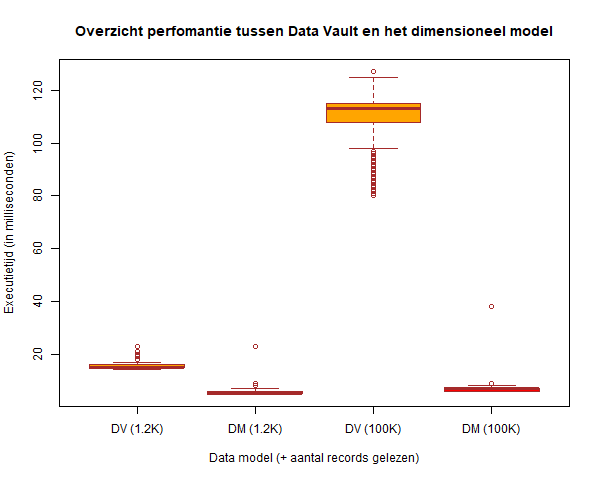
\includegraphics[scale=0.6]{../images/Score_perf.png}
	\caption{Boxplot van de uitvoeringstijden bij leesopdrachten van Data Vault en het dimensioneel model. }
	\label{fig:boxplotperf}
\end{figure}

Uit deze boxplot kan afgeleid worden dat er een kleine spreiding is van de resultaten bij het dimensioneel model (op enkele uitschieters na). Opmerkelijk is dat de executietijd bij Data Vault bij het opvragen van 100.000 records opmerkelijk hoger ligt en er meer spreiding bij de data is in vergelijking met de executietijd bij het opvragen van 100.000 records bij het dimensioneel model.

\subsection{Analyse van de resultaten}

De resultaten die verkregen zijn zullen onderworpen worpen aan een statistische toets (t-toets aangezien de standaardafwijking van de populatie niet gekend is). Bij de resultaten tussen Data Vault en het dimensioneel model (bij een dataset van 1200 records) zijn volgende hypotheses bepaald:

\[
H_0 = \mu_1 - \mu_2 = 0
\]
\[
H_1 = \mu_1 - \mu_2 > 0
\]

waarbij
$\mu_1$ = gemiddelde executietijd bij Data Vault met 1.200 records \&
$\mu_2$ = gemiddelde executietijd bij dimensioneel model met 1.200 records.

Er wordt een linkszijdige toets uitgevoerd omdat Data Vault veel meer joins bevat dan het dimensioneel model en dit zal een negatieve invloed hebben op het ophalen van de data. De vraag luidt of de resultaten significant zullen verschillen ten opzichte van het dimensioneel model.

Het betrouwbaarheidsinterval dat zal gehanteerd worden in deze toets is 95\%. Dit betekent dat met 95\% zekerheid
kan gezegd worden dat een bepaalde parameter binnen het
betrouwbaarheidsinterval zal liggen.

\[
\alpha = 1 - 0.95
\]
\[
\alpha = 0.05
\]

Het uitvoeren van de Welch Two Sample t-test in RStudio geeft volgend resultaat:

\begin{figure}[h]
	\centering
	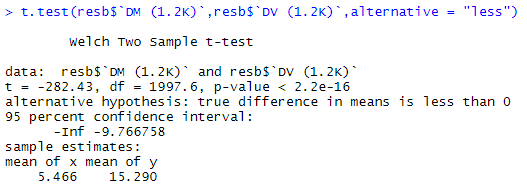
\includegraphics[scale=0.7]{../images/Ttest1200.png}
	\caption{Resultaat van de Welch Two Sample t-test in Rstudio voor de dataset met 1200 records tussen Data Vault en het dimensioneel model. }
	\label{fig:ttest1200}
\end{figure}

Aangezien de p-value uit de Welch Two Sample t-test (figuur \ref{fig:ttest1200}) kleiner is dan $\alpha$ betekent dit dat de nullhypothese mag verworpen worden en dat de alternative hypothese mag aanvaard worden.

Wanneer er dezelfde methodologie wordt toegepast voor het bepalen ofdat er een significant verschil aanwezig tussen Data Vault en het dimensioneel model bij een dataset van 100.000 records, bekomen we volgend resultaat:

\begin{figure}[h]
	\centering
	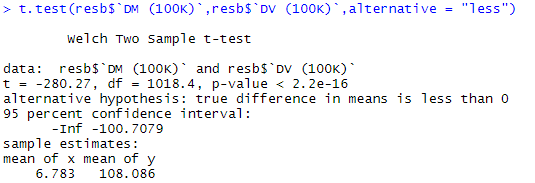
\includegraphics[scale=0.7]{../images/Ttest100000.png}
	\caption{Resultaat van de Welch Two Sample t-test in Rstudio voor de dataset met 100.000 records tussen Data Vault en het dimensioneel model. }
	\label{fig:ttest100000}
\end{figure}

Na het uitvoeren van deze test (figuur \ref{fig:ttest100000}) is de p-value hier ook kleiner dan $\alpha$, ook hier betekent dit dat er een significant verschil aanwezig is tussen de performantie van beide data modellen.

\subsubsection{Conclusie}
Er kan geconcludeerd worden dat er toch wel degelijk een significant verschil zit tussen de gemiddelde executietijd van een leesopdracht bij Data Vault in vergelijking met het dimensioneel model. Niet alleen het data model, maar ook de hoeveelheid data aanwezig in de tabellen van een data model heeft een invloed op de snelheid van leesoperaties. Het dimensioneel model gaat hiermee duidelijk veel beter om dan het Data Vault model. 

\section{Complexiteit}
Bij het modelleren van data kan complexiteit ontstaan zowel bij het interpreteren van het data model als bij het opmaken van het data model. 

Wanneer de business of de IT een dimensioneel model moet interpreteren, zal dit gemakkelijker gaan in vergelijking met een Data Vault model. Bij een dimensioneel model zijn veel minder relaties, dat zorgt voor een overzichtelijker schema. Ook komt alles samen in één centraal punt (fact), waaraan alles gelinkt is. Bij het interpreteren van een Data Vault model, moet die persoon al beschikken over kennis over Data Vault. Hij/zij moet weten wat het doel is van de verschillende soorten tabellen (hubs, links \& sattelites). Ook zullen de vele verschillende entiteiten samen het overzicht belemmeren. 

De transactionele gegevens staan bij het dimensioneel model altijd gecentraliseerd op één plaats. Zo is het zeer eenvoudig om te weten te komen welke transactionele gegevens (en business logica) er gebruikt wordt. Dit is niet altijd het geval bij Data Vault. In dit onderzoek staan die gegevens toevallig wel samen op één plaats, maar in de praktijk zal dit niet altijd het geval zijn. Dan worden de transactionele gegevens bij een Data Vault model samengevoegd in een data mart.

Als een datamodel ontworpen wordt aan de hand van het dimensioneel modelleren, kan er snel en gemakkelijk tot een resultaat bekomen worden in vergelijking met Data Vault. Bij het ontwerpen van een dimensioneel model wordt er gestart vanuit de dimensions, die leiden naar één centraal punt, de fact. Wanneer een Data Vault model dient ontworpen te worden, kan dit op veel verschillende manieren gebeuren. Er wordt gestart vanuit hubs, die de pilaren vormen voor het model, daarna worden deze verbonden met elkaar aan de hand van links. Finaal wordt beslist welke sattelites zullen aangemaakt worden en aan welke hubs/links deze gekoppeld zullen worden.

Wanneer historisatie van data een requirement is, dan heeft Data Vault een streepje voor op het dimensioneel modelleren. Bij Data Vault zit historisatie al in het model geïntegreerd, bij het dimensioneel modelleren niet. Er kan geopteerd worden voor historisatie bij het dimensioneel modelleren door gebruik te maken van slow changing dimensions, maar dit verhoogt wel aanzienlijk de complexiteit van het model.

Op vlak van complexiteit, kan er geconcludeerd worden dat Data Vault een hogere complexiteit bevat in vergelijking met het dimensioneel model, zowel op het vlak van interpreteren van het model als het opstellen van een nieuw model.

\section{Flexibiliteit}
Bij het toevoegen van nieuwe requirements, moet er bij Data Vault nieuwe hub(s) ontworpen en geïmplementeerd worden samen met de daarbij horende links/sattelites. Indien daarbij nieuwe businesslogica wordt bijgevoegd, kan deze in de nieuwe sattelites geplaatst worden. 

\begin{figure}[h]
	\centering
	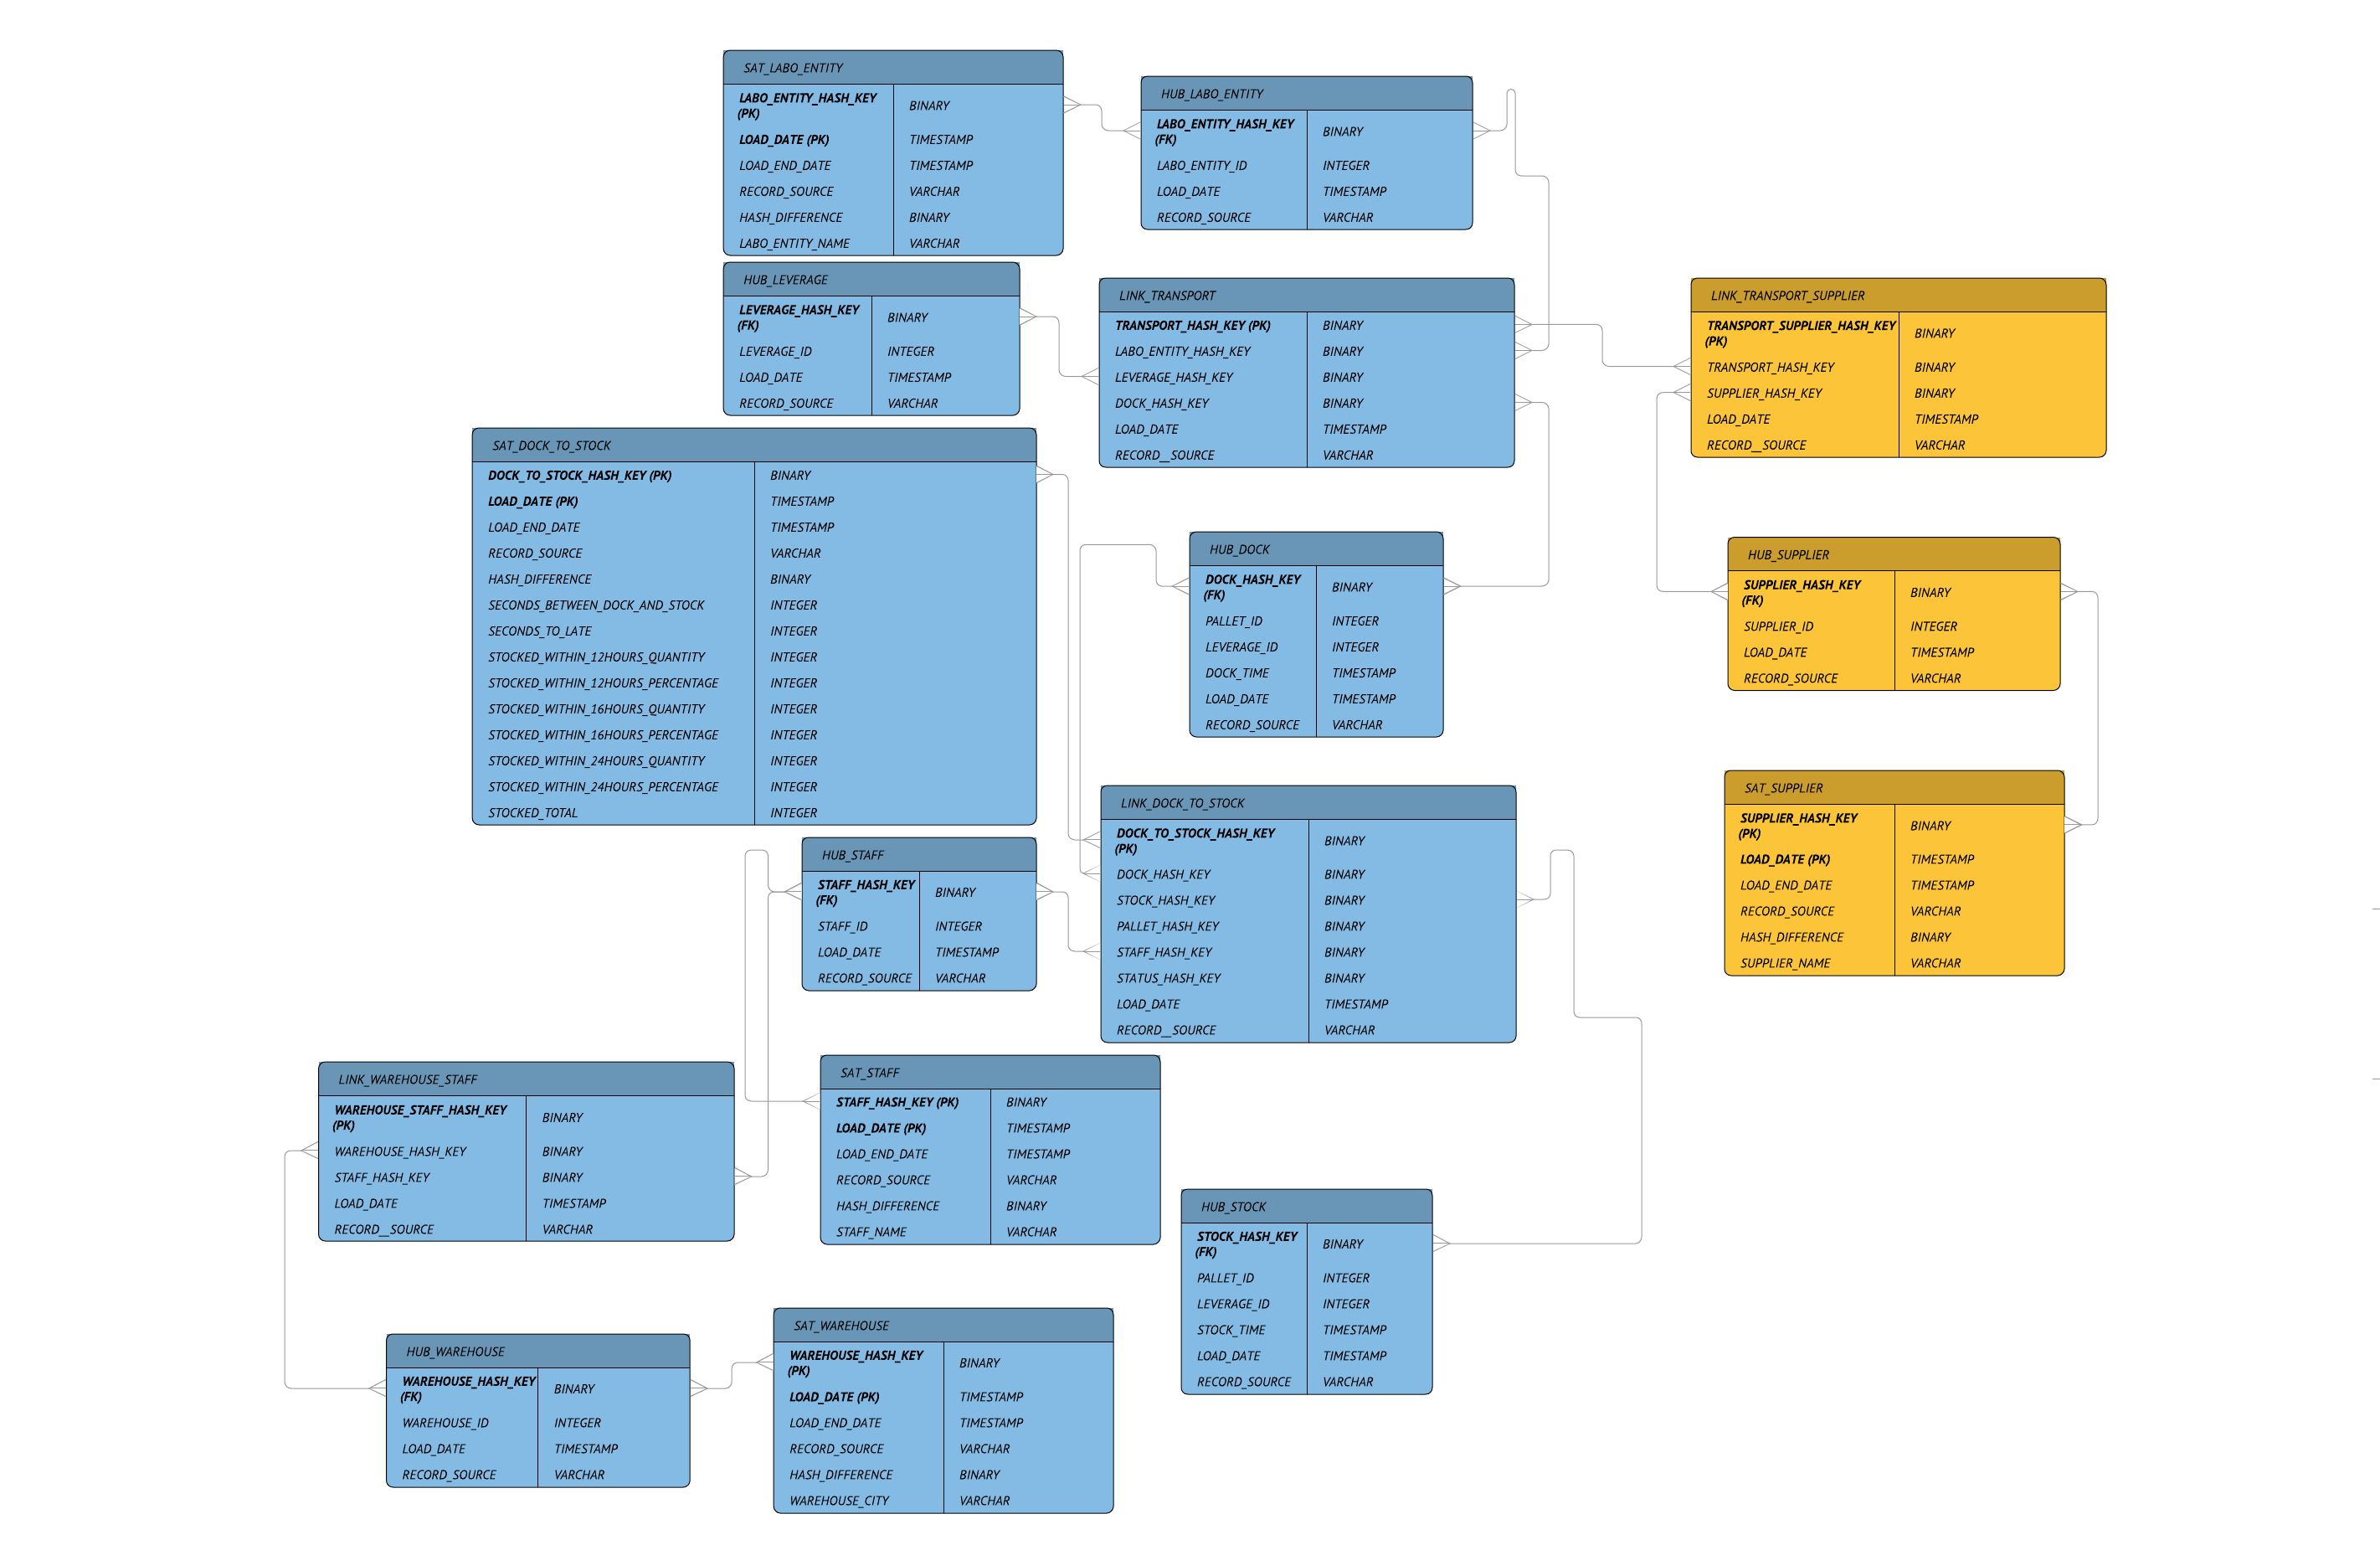
\includegraphics[scale=0.35]{../images/changedv.png}
	\caption{Het toevoegen van een nieuwe entiteit bij Data Vault (gemaakt via Lucidchart.com).}
	\label{fig:changedv}
\end{figure}

In figuur \ref{fig:changedv} wordt een nieuwe business requirement toegevoegd bij een bestaand Data Vault model. Hierbij wordt het bestaand model niet aangepast, maar er wordt wel een uitbreiding uitgevoerd. Er wordt een nieuwe link, hub \& sattelite toegevoegd (in het geel).

Deze manier van werken brengt een heel groot voordeel met zich mee op vlak van project management: via deze manier kan er gewerkt worden via de agile-manier, aangezien een toevoeging geen impact mag hebben op het bestaand data model.

Nieuwe business requirements toevoegen in het dimensioneel model is niet zo vanzelfsprekend. Een dimension ontwerpen en implementeren is eenvoudig, maar die nieuwe dimension zal moeten in relatie gezet worden met de centrale fact tabel. Dit betekent dat er een nieuwe key zal moeten toegevoegd worden in de fact tabel, en dat de huidige composite key dus zal moeten aangepast worden. De nieuwe toegevoegde key zal geen lege waarde mogen zijn.

\begin{figure}[h]
	\centering
	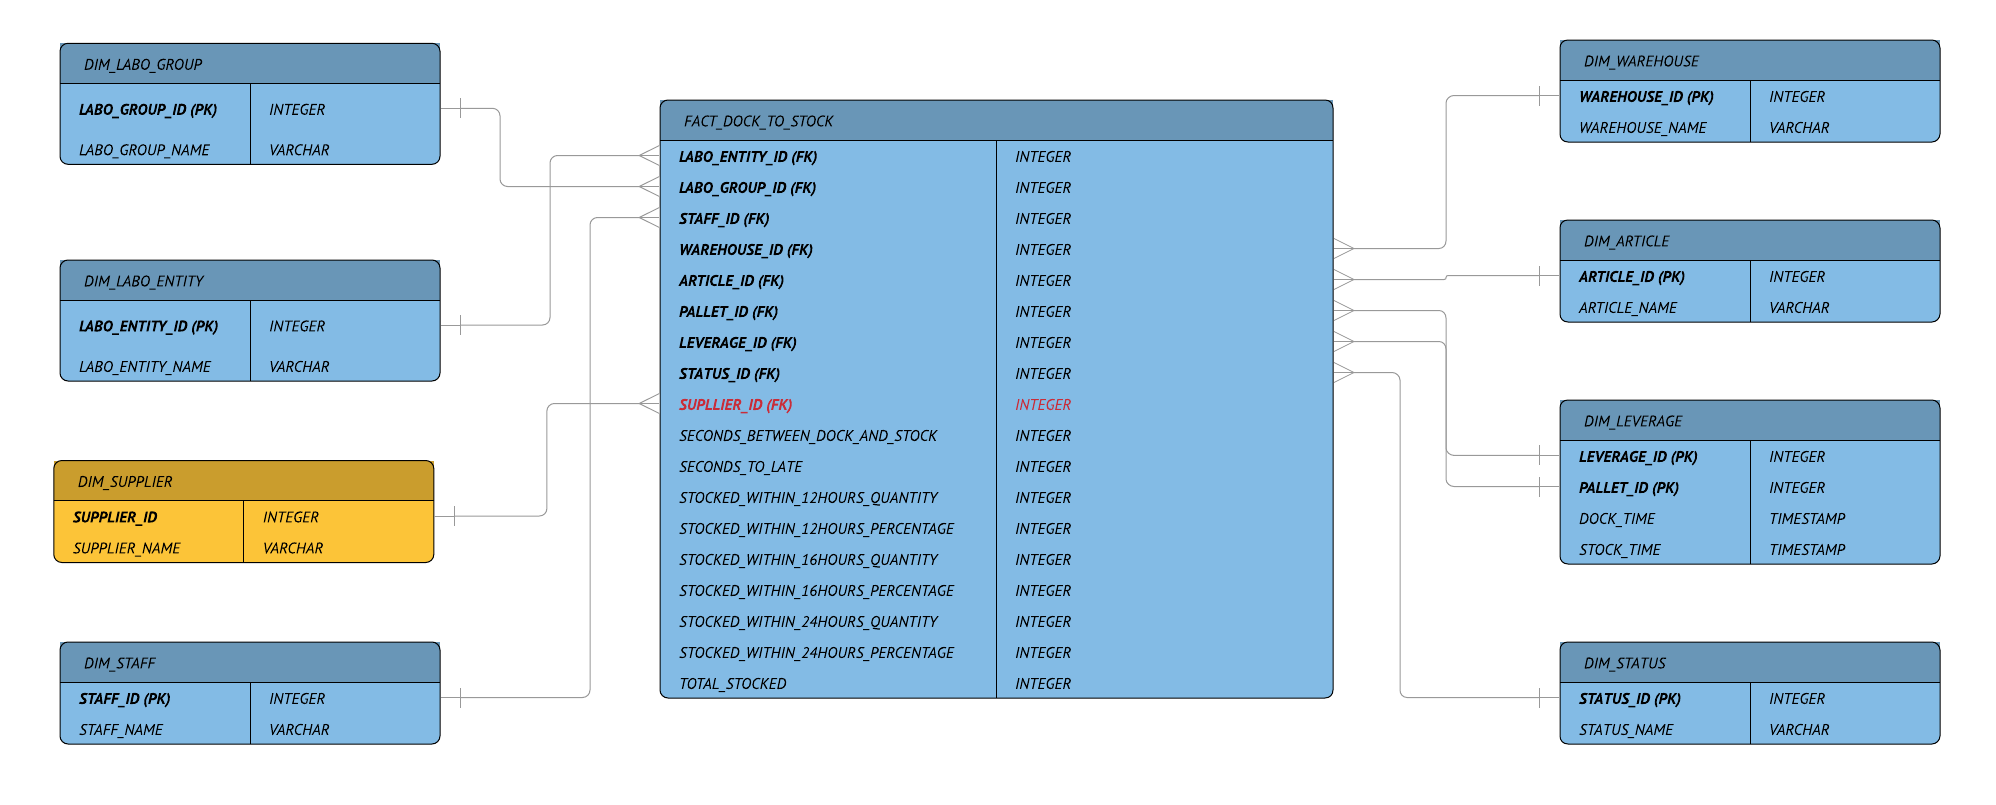
\includegraphics[scale=0.45]{../images/changedm.png}
	\caption{Het toevoegen van een nieuwe dimension bij een dimensioneel model (gemaakt via Lucidchart.com).}
	\label{fig:changedm}
\end{figure}

In figuur \ref{fig:changedm} wordt een nieuwe dimension (in het geel) toegevoegd aan het dimensioneel model. Het toevoegen van de nieuwe dimension heeft geen effect op de bestaande dimensions, maar wel in de fact tabel. In de fact tabel zal er een kolom moeten toegevoegd worden die de overeenkomstige keys bevat met de huidige data. Dit betekent dat het toevoegen van een nieuwe dimension wel degelijk een invloed heeft op het bestaande model en dat hier moeilijk via de agile methodologie kan gewerkt worden.

De structuur van een dimensioneel model ligt vast. Er is altijd een fact tabel die alle dimensions met elkaar verbindt. Het biedt geen opportuniteit om het schema te ontwerpen op basis van een business proces. Bij Data Vault is dit echter wel mogelijk. De flexibiliteit in de opbouw van een Data Vault is enorm hoog. Zo kan het model ontworpen worden op basis van een proces.

In een Data Vault model worden alleen maar many-to-many relaties gelegd door gebruik te maken van links. Dit is niet het geval bij het dimensioneel model. Door te werken met many-to-many relaties, verhoogt dit de flexibiliteit. Het nadeel door met many-to-many relaties te werken is dat het opvragen data langzamer zal verlopen.

Het toevoegen van nieuwe bron gebeurt doorgaans ook eenvoudig bij Data Vault. Hiervoor moeten enkel nieuwe sattelites aangemaakt worden voor de benodigde data. Deze sattelites worden dan verbonden met de bijhoorende hubs. Opnieuw wordt het bestaande model niet aangepast. Bij het dimensioneel model moet hiervoor gebruik gemaakt worden van slow changing dimensions. Als dit principe niet van in het begin opgenomen is in het model, dan zal er heel wat moeite moeten gestopt worden in het toevoegen van een nieuwe databron (extra kolommen aanmaken, bestaande ETL aanpassen, ...).

De conclusie bij de vergelijking van Data Vault en het dimensioneel op basis van flexibiliteit is zeer duidelijk. De grote winnaar bij flexibiliteit is Data Vault, dat op alle vlakken van dit aspect duidelijk de betere keuze is.

\section{Schaalbaarheid}
Data warehouses bevatten doorgaans enorme hoeveelheden data. Bij de vergelijking tussen Data Vault en het dimensioneel model is het belangrijk om de schaalbaarheid van beide modellen te bestuderen. 

Het inladen van data in data warehouses kan bij enorme hoeveelheden data enorm veel tijd in beslag nemen. Daarom is het een enorm voordeel indien er kan gebruik gemaakt worden van parallel inladen, wat het geval is bij Data Vault en niet bij het dimensioneel modelleren.

Bij het inladen van data in het Data Vault model zijn alle tabellen onafhankelijk, dit wil zeggen dat alle tabellen tegelijk kunnen worden ingeladen. Bij het dimensioneel model moeten eerst de dimensions ingeladen zijn vooraleer de fact tabel kan ingeladen/aangevuld worden.

In deze sectie zullen 1000 keer 1 record ingeladen worden in alle tabellen van beide datamodellen. Hierbij worden de uitvoeringstijden van beide data modellen bijgehouden en vervolgens wordt een analyse opgemaakt op basis van de resultaten.

\subsection{Procedure} 
\begin{lstlisting}[frame=single] 
ALTER PROCEDURE "TESTJORIK_BV"."ADDDATA" LANGUAGE SQLSCRIPT AS BEGIN
DECLARE START_TIME_DV timestamp;
DECLARE END_TIME_DV timestamp;
DECLARE TIME_DIFF_DV int;
DECLARE START_TIME_DM timestamp;
DECLARE END_TIME_DM timestamp;
DECLARE TIME_DIFF_DM int;
DECLARE EXEC_ID int;
DECLARE AANTAL int;

EXEC_ID = 1002;
DELETE FROM "TESTJORIK_BV"."UITVOERINGSTIJDEN";
WHILE :EXEC_ID < 2002 DO
INSERT INTO "TESTJORIK_BV"."UITVOERINGSTIJDEN" ("EXEC_ID") VALUES (:EXEC_ID);

UPDATE "TESTJORIK_BV"."UITVOERINGSTIJDEN" SET "START_TIME_DV" = CURRENT_TIMESTAMP
WHERE "EXEC_ID" = :EXEC_ID;

--add
BEGIN PARALLEL EXECUTION

UPSERT "BP_DHLPL_RAWDATAVAULT"."LINK_DOCK_TO_STOCK" VALUES (HASH_SHA256(TO_BINARY(:EXEC_ID)),CURRENT_TIMESTAMP,'dummy','1B3E2CAC1E858C5C078BE89E8DB166CA019A 2C281C1971925C6AC7CFFFCE1EBC', '92F061FC6C9BC77EBAB163C6 3118347701E3825928FF6A8FE75736DBCB0A4CB1',
'27BADC983DF1780B60C2B3FA 9D3A19A00E46AAC798451F0FEBDCA52920FAADDF','7902699BE42C8A8E46FBBB45017 26517E86B22C56A189F7625A6DA49081B2451', '4E07408562BEDB8B60CE05C1DECF E3AD16B72230967DE01F640B7E4729B49FCE');
UPSERT "BP_DHLPL_RAWDATAVAULT"."SAT_DOCK_TO_STOCK" VALUES (HASH_SHA256(TO_BINARY(:EXEC_ID)),CURRENT_TIMESTAMP,CURRENT_TIMESTAMP,'dummy','1',1,1,1,1,1,1,1,1,1);
UPSERT "BP_DHLPL_RAWDATAVAULT"."SAT_LABO_ENTITY" VALUES (HASH_SHA256(TO_BINARY(:EXEC_ID)),CURRENT_TIMESTAMP,CURRENT_TIMESTAMP,'dummy','1','naam');
UPSERT "BP_DHLPL_RAWDATAVAULT"."SAT_LABO_GROUP" VALUES (HASH_SHA256(TO_BINARY(:EXEC_ID)),CURRENT_TIMESTAMP,CURRENT_TIMESTAMP,'dummy','1','naam');
UPSERT "BP_DHLPL_RAWDATAVAULT"."SAT_STATUS" VALUES (HASH_SHA256(TO_BINARY(:EXEC_ID)),CURRENT_TIMESTAMP,CURRENT_TIMESTAMP,'dummy','1','naam');
UPSERT "BP_DHLPL_RAWDATAVAULT"."SAT_STAFF" VALUES (HASH_SHA256(TO_BINARY(:EXEC_ID)),CURRENT_TIMESTAMP,CURRENT_TIMESTAMP,'dummy','1','naam');
UPSERT "BP_DHLPL_RAWDATAVAULT"."SAT_WAREHOUSE" VALUES (HASH_SHA256(TO_BINARY(:EXEC_ID)),CURRENT_TIMESTAMP,CURRENT_TIMESTAMP,'dummy','1','naam');
UPSERT "BP_DHLPL_RAWDATAVAULT"."SAT_ORDERLINE" VALUES (HASH_SHA256(TO_BINARY(:EXEC_ID)),CURRENT_TIMESTAMP,CURRENT_TIMESTAMP,'dummy','1',1);
UPSERT "BP_DHLPL_RAWDATAVAULT"."SAT_ARTICLE" VALUES (HASH_SHA256(TO_BINARY(:EXEC_ID)),CURRENT_TIMESTAMP,CURRENT_TIMESTAMP,'dummy','1','naam');
UPSERT "BP_DHLPL_RAWDATAVAULT"."HUB_LABO_ENTITY" VALUES (HASH_SHA256(TO_BINARY(:EXEC_ID)),:EXEC_ID,CURRENT_TIMESTAMP,'dummy');
UPSERT "BP_DHLPL_RAWDATAVAULT"."HUB_LABO_GROUP" VALUES (HASH_SHA256(TO_BINARY(:EXEC_ID)),:EXEC_ID,CURRENT_TIMESTAMP,'dummy');
UPSERT "BP_DHLPL_RAWDATAVAULT"."HUB_STATUS" VALUES (HASH_SHA256(TO_BINARY(:EXEC_ID)),:EXEC_ID,CURRENT_TIMESTAMP,'dummy');
UPSERT "BP_DHLPL_RAWDATAVAULT"."HUB_STAFF" VALUES (HASH_SHA256(TO_BINARY(:EXEC_ID)),:EXEC_ID,CURRENT_TIMESTAMP,'dummy');
UPSERT "BP_DHLPL_RAWDATAVAULT"."HUB_WAREHOUSE" VALUES (HASH_SHA256(TO_BINARY(:EXEC_ID)),:EXEC_ID,CURRENT_TIMESTAMP,'dummy');
UPSERT "BP_DHLPL_RAWDATAVAULT"."HUB_ARTICLE" VALUES (HASH_SHA256(TO_BINARY(:EXEC_ID)),:EXEC_ID,CURRENT_TIMESTAMP,'dummy');
UPSERT "BP_DHLPL_RAWDATAVAULT"."HUB_PALLET" VALUES (HASH_SHA256(TO_BINARY(:EXEC_ID)),:EXEC_ID,CURRENT_TIMESTAMP,'dummy');
UPSERT "BP_DHLPL_RAWDATAVAULT"."HUB_DELIVERY" VALUES (HASH_SHA256(TO_BINARY(:EXEC_ID)),:EXEC_ID,CURRENT_TIMESTAMP,'dummy');
UPSERT "BP_DHLPL_RAWDATAVAULT"."HUB_DOCK" VALUES (HASH_SHA256(TO_BINARY(:EXEC_ID)),:EXEC_ID,:EXEC_ID,CURRENT_TIMESTAMP,CURRENT_TIMESTAMP, 'dummy');
UPSERT "BP_DHLPL_RAWDATAVAULT"."HUB_STOCK" VALUES (HASH_SHA256(TO_BINARY(:EXEC_ID)),:EXEC_ID,:EXEC_ID,CURRENT_TIMESTAMP,CURRENT_TIMESTAMP, 'dummy');
UPSERT "BP_DHLPL_RAWDATAVAULT"."LINK_ORDERLINE" VALUES (HASH_SHA256(TO_BINARY(:EXEC_ID)),CURRENT_TIMESTAMP,'dummy','1','1');
UPSERT "BP_DHLPL_RAWDATAVAULT"."LINK_LABO_ENTITY_GROUP" VALUES (HASH_SHA256(TO_BINARY(:EXEC_ID)),CURRENT_TIMESTAMP,'dummy','1','1');
UPSERT "BP_DHLPL_RAWDATAVAULT"."LINK_TRANSPORT" VALUES (HASH_SHA256(TO_BINARY(:EXEC_ID)),CURRENT_TIMESTAMP,'dummy','1','1','1');
UPSERT "BP_DHLPL_RAWDATAVAULT"."LINK_WAREHOUSE_STAFF" VALUES (HASH_SHA256(TO_BINARY(:EXEC_ID)),CURRENT_TIMESTAMP,'dummy','1','1');
END;

UPDATE "TESTJORIK_BV"."UITVOERINGSTIJDEN" SET "END_TIME_DV" = CURRENT_TIMESTAMP
WHERE "TESTJORIK_BV"."UITVOERINGSTIJDEN"."EXEC_ID" = :EXEC_ID;
UPDATE "TESTJORIK_BV"."UITVOERINGSTIJDEN" SET "START_TIME_DM" = CURRENT_TIMESTAMP
WHERE "TESTJORIK_BV"."UITVOERINGSTIJDEN"."EXEC_ID" = :EXEC_ID;

--dimmodel
BEGIN PARALLEL EXECUTION
UPSERT "BP_DHLPL_DATAWAREHOUSELAAG"."DIM_LABO_GROUP" VALUES (:EXEC_ID,'x');
UPSERT "BP_DHLPL_DATAWAREHOUSELAAG"."DIM_LABO_ENTITY" VALUES (:EXEC_ID,'x');
UPSERT "BP_DHLPL_DATAWAREHOUSELAAG"."DIM_STAFF" VALUES (:EXEC_ID,'x');
UPSERT "BP_DHLPL_DATAWAREHOUSELAAG"."DIM_WAREHOUSE" VALUES (:EXEC_ID,'x');
UPSERT "BP_DHLPL_DATAWAREHOUSELAAG"."DIM_ARTICLE" VALUES (:EXEC_ID,'x');
UPSERT "BP_DHLPL_DATAWAREHOUSELAAG"."DIM_STATUS" VALUES (:EXEC_ID,'x');
UPSERT "BP_DHLPL_DATAWAREHOUSELAAG"."DIM_DELIVERY" VALUES (:EXEC_ID,:EXEC_ID,CURRENT_TIMESTAMP,CURRENT_TIMESTAMP);
END;
UPSERT "BP_DHLPL_DATAWAREHOUSELAAG"."FACT_DOCKTOSTOCK" VALUES (1,1,1,1,1,1,:EXEC_ID,1,1,1,1,1,1,1,1);

UPDATE "TESTJORIK_BV"."UITVOERINGSTIJDEN" SET "END_TIME_DM" = CURRENT_TIMESTAMP
WHERE "TESTJORIK_BV"."UITVOERINGSTIJDEN"."EXEC_ID" = :EXEC_ID;

UPDATE "TESTJORIK_BV"."UITVOERINGSTIJDEN" SET "DIFF_TIME_DV" = (NANO100_BETWEEN(START_TIME_DV,END_TIME_DV) / 10000)
WHERE "TESTJORIK_BV"."UITVOERINGSTIJDEN"."EXEC_ID" = :EXEC_ID;

UPDATE "TESTJORIK_BV"."UITVOERINGSTIJDEN" SET "DIFF_TIME_DM" = (NANO100_BETWEEN(START_TIME_DM,END_TIME_DM) / 10000)
WHERE "TESTJORIK_BV"."UITVOERINGSTIJDEN"."EXEC_ID" = :EXEC_ID;
EXEC_ID = :EXEC_ID + 1;
END WHILE;
END;
\end{lstlisting}

\subsection{Resultaten}
In tabel \ref{tab:spgups} wordt een overzicht weergegeven van de steekproefgemiddelden met de daarbijhorende standaardafwijking van de executietijd bij het uitvoeren van de UPSERT-operatie bij beide modellen.

\begin{center}
	\renewcommand{\arraystretch}{2}%
	\begin{longtable}{  l  p{4,5cm}  p{4,5cm} }
		\ & \textbf{Data Vault} & \textbf{Dimensioneel model} \\ \hline
		\textbf{1 record / tabel} & 3.109 ms (\sigma = 1.438) & 3.411 ms (\sigma = 0.781) \\
		\caption{Overzicht van het steekproefgemiddelde bij Data Vault en het dimensioneel model bij het wegschrijven van data naar elke tabel.}
		\label{tab:spgups}
	\end{longtable}
\end{center}

Het verschil tussen de gemiddelde executietijden voor het invoegen van data is niet erg groot. Deze waarden zullen moeten onderworpen worden aan een statistische toets om te bepalen of er een significant verschil is.

\begin{figure}[H]
	\centering
	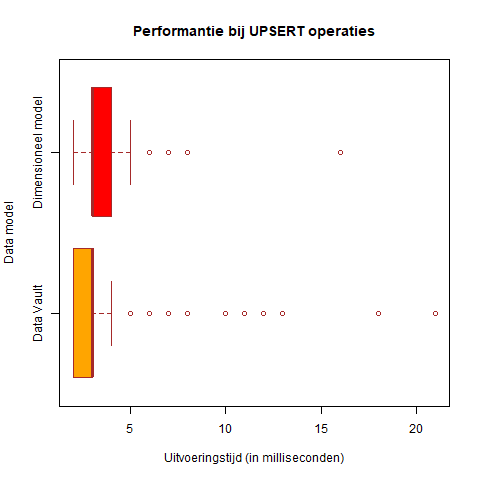
\includegraphics[scale=0.6]{../images/Score_upsert.png}
	\caption{Boxplot van de uitvoeringstijden bij UPSERT-operaties van Data Vault en het dimensioneel model. }
	\label{fig:boxplotupsert}
\end{figure}

In figuur \ref{fig:boxplotupsert} wordt een boxplot weergegeven. Op deze figuur merken we op dat er een kleine spreiding is van de data bij beide data modellen, op enkele uitschieters na. De gemiddelde executietijd ligt dicht bij elkaar.

\subsection{Analyse van de resultaten}
Ook in deze subsectie zullen de resultaten die verkregen zijn onderworpen worpen aan een statistische toets (t-toets aangezien de standaardafwijking van de populatie niet gekend is). Volgende hypothesen worden opgemaakt:

\[
H_0 = \mu_1 - \mu_2 = 0
\]
\[
H_1 = \mu_1 - \mu_2 \neq 0
\]

waarbij
$\mu_1$ = gemiddelde executietijd bij Data Vault voor het toevoegen van een record bij elke tabel van het model \&
$\mu_2$ = gemiddelde executietijd bij dimensioneel model voor het toevoegen van een record bij elke tabel van het model.

Het betrouwbaarheidsinterval dat zal gehanteerd worden in deze toets is ook 95\%.

\[
\alpha = 1 - 0.95 = 0.05
\]


Het uitvoeren van de Welch Two Sample t-test in RStudio geeft volgend resultaat:

\begin{figure}[H]
	\centering
	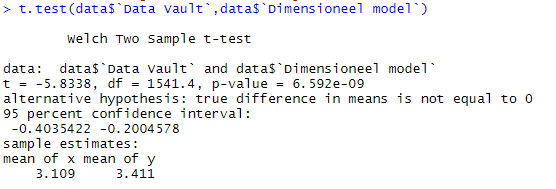
\includegraphics[scale=0.7]{../images/Ttestupsert.png}
	\caption{Resultaat van de Welch Two Sample t-test in Rstudio voor het verschil in uitvoeringstijden bij een UPSERT-operatie. }
	\label{fig:ttestups}
\end{figure}

Aangezien de p-value uit figuur \ref{fig:ttestups} kleiner is dan $\alpha$ betekent dit dat ook deze nullhypothese mag verworpen worden en dat de alternative hypothese mag aanvaard worden. Er is dus een significant verschil aanwezig tussen beide data modellen bij het inladen van data.

\subsection{Conclusie} 

Bij Data Vault kan de data significant sneller in het model geladen worden dan bij het dimensioneel model. Dit heeft te maken met het feit dat er bij het dimensioneel model eerst de dimensions moeten ingeladen zijn vooraleer de fact tabel kan ingeladen worden. Data Vault maakt gebruik van hash keys, hierdoor kan er sneller gecontroleerd worden of een bepaalde record al aanwezig is.

\section{Audit}
Het bijhouden van historisatie en extra informatie over gegevens is voor sommige organisaties van groot belang. Denk maar bijvoorbeeld aan de banksector, indien er iets fout is gelopen met een bepaalde transactie of indien men wil te weten komen van waar bepaalde data opgehaald wordt, moet er hiervoor extra informatie aangeleverd kunnen worden. Historisatie wordt voornamelijk gebruikt bij gevoelige data. Andere voorbeelden van sectoren zijn: medische sector, overheden, verzekeringen, ....

In de Data Vault methodologie zit historisatie verwerkt. Er wordt extra informatie bijgehouden over waar de data exact vandaan komt (RECORD\_SOURCE), en wanneer de extractie van die data uit de bron gebeurd is (LOAD\_DATE). De reden waarom het tijdstip van extractie wordt bijgehouden en niet het tijdstip van het inladen van de gegevens in de data warehouse is omdat het ETL proces zeer lang kan duren en in de tussentijd de data in het bronsysteem al gewijzigd kan zijn. Via de Data Vault methodologie worden er in principe geen rijen gewijzigd (enkel de kolom LOAD\_END\_DATE), en worden nieuwere versies van data gewoon toegevoegd in de databank.

Bij het dimensioneel model wordt standaard noch de historisatie van data, noch extra informatie over de aangeleverde data niet bijgehouden. Voor historisatie bij het dimensioneel model kan gebruik gemaakt worden van slow changing dimensions. Indien gewenst kan er natuurlijk ook altijd geopteerd worden om deze extra informatie op te nemen door enkele kolommen toe te voegen. 

Er kan geconcludeerd worden dat Data Vault standaard historisatie toepast in hun model en dat er extra informatie (audit data) opgeslaan wordt over de data. Bij het dimensioneel model worden historisatie en het bijhouden van audit data niet opgenomen, maar het kan wel geïmplementeerd worden indien gewenst.

\newpage
\section{Overzicht}
In tabel \ref{tab:overzicht} wordt een overzicht weergegeven van de verschillen op basis van de 5 pijlers.
\begin{center}
	\renewcommand{\arraystretch}{2}%
	\begin{longtable}{  l  p{5,5cm}  p{5,5cm} }
		\ & \textbf{Data Vault} & \textbf{Dimensioneel model} \\ \hline
		Performantie & Data opvragen gebeurt significant langzamer door de vele joins in het model. & Data lezen gebeurt vlot door een beperkt aantal joins. \\ \hline
		Complexiteit & Hoge complexiteit, kennis nodig rond Data Vault. & Lage complexiteit, overzichtelijk. \\ \hline
		Flexibiliteit & Zeer hoge flexibiliteit, mogelijk om via de agile methode te werken. & Zeer lage flexibiliteit, vaste structuur. \\ \hline
		Schaalbaarheid & Goede schaalbaarheid door parallel inladen van de data. & Data inladen kan significant langer duren doordat de fact tabel afhankelijk is van de dimensions en er niet parallel kan ingeladen worden.  \\ \hline
		Audit & Extra informatie aanwezig en de historiek van de data wordt bijgehouden. & Extra informatie niet aanwezig, indien gewenst kan dit wel toegevoegd worden. \\
		\caption{Overzicht van het vergelijkend onderzoek.}
		\label{tab:overzicht}
	\end{longtable}
\end{center}